%%%%%%%%%%%%%%%%%%%%%%%%%%%%%%%%%%%%%%%%%%%%%%%%%%%%%%%%%%%%%%%%%%%%%%%%%%%%%%%
% Chapter 'Adsorption - Isobutane - mof powder cubtc'
%%%%%%%%%%%%%%%%%%%%%%%%%%%%%%%%%%%%%%%%%%%%%%%%%%%%%%%%%%%%%%%%%%%%%%%%%%%%%%%
\subsection{Mof powder cubtc}
%
%%%%%%%%%%%%%%%%%%%%%%%%%%%%%%%%%%%%%%%%%%%%%%%%%%%%%%%%%%%%%%%%%%%%%%%%%%%%%%%
%%%%%%%%%%%%%%%%%%%%%%%%%%%%%%%%%%%%%%%%%%%%%%%%%%%%%%%%%%%%%%%%%%%%%%%%%%%%%%%
\subsubsection{DualSiteSips - ID 1}
%
\begin{tabular}[l]{|lp{11.5cm}|}
\hline
\addlinespace

\textbf{Sorbent:} & mof powder \\
\textbf{Subtype:} & cubtc \\
\textbf{Refrigerant:} & Isobutane \\
\textbf{Equation:} & DualSiteSips \\
\textbf{ID:} & 1 \\
\textbf{Reference:} & Lamia, Nabil; Jorge, Miguel; Granato, Miguel A.; Almeida Paz, Filipe A.; Chevreau, Hubert; Rodrigues, Alírio E. (2009): Adsorption of propane, propylene and isobutane on a metal–organic framework. Molecular simulation and experiment. In: Chemical Engineering Science 64 (14), S. 3246–3259. DOI: 10.1016/j.ces.2009.04.010. \\
\textbf{Comment:} & None \\

\addlinespace
\hline
\end{tabular}
\newline

\textbf{Properties of sorbent:}
\newline
%
\begin{longtable}[l]{lll}
\toprule
\addlinespace
\textbf{Property} & \textbf{Unit} & \textbf{Value} \\
\addlinespace
\midrule
\endhead
\bottomrule
\endfoot
\bottomrule
\endlastfoot
\addlinespace

Diameter of crystal & \si{\milli\meter} & 0.0016\\
Surface area & \si{\square\meter\per\gram} & 1500-2100\\
Bulk density & \si{\kilogram\per\cubic\meter} & 350\\

\addlinespace\end{longtable}

\textbf{Equation and parameters:}
\newline
%
Loading $w$ in $\si{\kilogram\per\kilogram}$ is calculated depending on pressure $p$ in $\si{\pascal}$ and temperature $T$ in $\si{\kelvin}$ by:
%
\begin{equation*}
\begin{split}
w &=& \sum_{i=A}^{B} w_\mathrm{i} \frac{\left( b_i p \right) ^ {\nicefrac{1}{\eta_i}} }{1 + \left( b_i p \right) ^ {\nicefrac{1}{\eta_i}}} & \quad\text{, and} \\
b_i &=& b_{i,0} \exp \left( \frac{Q_i}{R T} \left( 1 - \frac{T}{T_0} \right) \right) & \quad\text{.}
\end{split}
\end{equation*}
%
The parameters of the equation are:
%
\begin{longtable}[l]{lll|lll}
\toprule
\addlinespace
\textbf{Par.} & \textbf{Unit} & \textbf{Value} &	\textbf{Par.} & \textbf{Unit} & \textbf{Value} \\
\addlinespace
\midrule
\endhead

\bottomrule
\endfoot
\bottomrule
\endlastfoot
\addlinespace

$b_\mathrm{A,0}$ & $\si{\per\pascal}$ & 8.200000000e-04 & $b_\mathrm{B,0}$ & $\si{\per\pascal}$ & 6.000000000e-05 \\
$Q_\mathrm{A}$ & $\si{\joule\per\mole}$ & 3.790000000e+04 & $Q_\mathrm{B}$ & $\si{\joule\per\mole}$ & 4.080000000e+04 \\
$\eta_\mathrm{A}$ & - & 5.500000000e-01 & $\eta_\mathrm{B}$ & - & 1.000000000e+00 \\
$w_\mathrm{A}$ & $\si{\kilogram\per\kilogram}$ & 2.975744000e-01 & $w_\mathrm{B}$ & $\si{\kilogram\per\kilogram}$ & 6.393200000e-02 \\
$T_0$ & $\si{\kelvin}$ & 3.230000000e+02 & & & \\

\addlinespace\end{longtable}

\textbf{Validity:}
\newline
Equation is approximately valid for $581.5 \si{\pascal} \leq p \leq 99177.0 \si{\pascal}$,  $323.0 \si{\kelvin} \leq T \leq 423.0 \si{\kelvin}$, and $0.011061398 \si{\kilogram\per\kilogram} \leq w \leq 0.349172174 \si{\kilogram\per\kilogram}$.
\newline

\textbf{Visualization:}
%
\begin{figure}[!htp]
{\noindent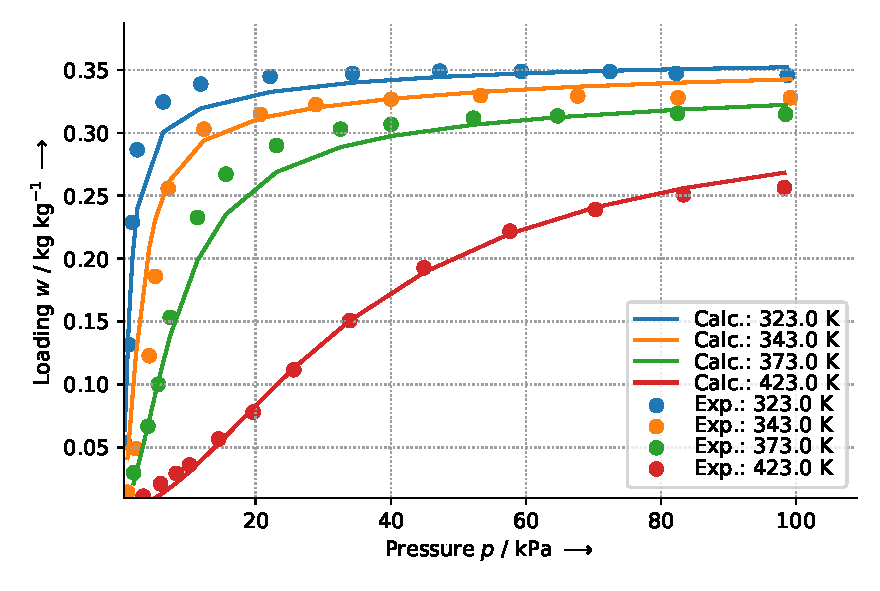
\includegraphics[height=10cm, keepaspectratio]{figs/ads/ads_Isobutane_mof_powder_cubtc_DualSiteSips_1.pdf}}
\end{figure}
%

To generate the figure, the following refrigerant functions were selected:
\begin{itemize}
\item Vapor pressure: VaporPressure\_EoS1 - ID 1
\item Saturated liquid density: SaturatedLiquidDensity\_EoS1 - ID 1
\end{itemize}

The uncertainity of the experimental data is:
\begin{itemize}
\item Data source $\,\to\,$ Data was taken from figure
\item Pressure, absolute, in $\si{\pascal}$ $\,\to\,$ 50
\item Temperature, absolute, in $\si{\kelvin}$ $\,\to\,$ 0.1
\end{itemize}

The mean absolute percentage error (MAPE) between the experimental and calculated data results in 15.25\%.
\FloatBarrier
\newpage
%%%%%%%%%%%%%%%%%%%%%%%%%%%%%%%%%%%%%%%%%%%%%%%%%%%%%%%%%%%%%%%%%%%%%%%%%%%%%%%
